\chapter{Results}

I have tested the two algorithms described in \nameref{chap:design} using the structure given in \nameref{chap:implementation}.\\
There are two major parts which should be analyzed: the correctness of the algorithm and its running time.

\section{Correctness}

We have collected a set of $4500$ images from the Internet, which we have classified in about $1600$ similarity sets, each set being composed of up to five images. The images within a similarity set differ in size, having various watermarks and filters applied (these sets are known to be correct beforehand). We have inserted these images in a larger set of $100.000$ images taken from the Internet and performed queries for each of the $4500$ images of the similarity sets, getting the top $10$ similar images. We want to observe:
\begin{itemize}
	\item if the algorithm finds the exact match, i.e. the image that has been queried with
	\item if the algorithm finds the other images which are part of the same similarity set
	\item the mean running time of a query
	\item how varying the metrics described in \nameref{chap:design} above influences the results of the query
\end{itemize}

We evaluate the response to a query, by looking at the indices of the images from the current similarity set in the list of results returned by the query. Thus, the $index\ score$ for a certain query can be computed as the sum of these indices; the smaller the sum, the closer in the response list are the images we want to find. \\
For the set of $100.000$ images we use $P=20$ KD-trees, each KD-tree storing the descriptors for $N=5000$ images. The descriptors are computed for images which are resized to keep the aspect ratio (the third storing possibility described in \nameref{chap:implementation}).\\

The results of this test can be seen in the following two tables. The first one describes, for similarity sets of size $3$, $4$ and $5$, and for the metrics described in \nameref{chap:design}, the average number of how many of these images are found in the list of $10$ returned images.\\

\begin{table}[H]
\centering
\begin{tabular} {c | c | c | c}
	& max nr descs & min avg & max dist to avg \\
	\hline
	3 & 2.85 & 2.63 & 2.86 \\
	\hline
	4 & 3.85 & 3.55 & 3.85 \\
	\hline
	5 & 4.65 & 4.13 & 4.64 \\
\end{tabular}
\caption{Average number of found images for $P=20$ and $N=5000$}
\end{table}

The second table shows the $index\ score$ (described above) for the same queries and metrics.\\

\begin{table}[H]
\centering
\begin{tabular} {c | c | c | c}
	& max nr descs & min avg & max dist to avg \\
	\hline
	3 & 4.86 & 6.85 & 4.78 \\
	\hline
	4 & 7.87 & 10.24 & 7.85 \\
	\hline
	5 & 13.47 & 17.48 & 13.35 \\
\end{tabular}
\caption{$Index\ scores$ for $P=20$ and $N=5000$}
\end{table}

It can be observed that the third metric, the largest distance from the descriptors of an image to the average of all found descriptors, provides the best results.\\

\subsection{Fixed dimension image storing}
	We computed the descriptors for images resized to a fixed value (height $400$ and width $300$), and analyzed the same metrics and scores described above. The results can be seen in tables
\ref{table:fixDimension1} and \ref{table:fixDimension2}. These results confirm that this image storing
performs worse than the aspect-ratio one, so we have decided to continue using the first one.\\
	 
\begin{table}[H]
\centering
\begin{tabular} {c | c | c | c}
	& max nr descs & min avg & max dist to avg \\
	\hline
	3 & 2.69 & 2.08 & 2.73 \\
	\hline
	4 & 3.55 & 2.60 & 3.62 \\
	\hline
	5 & 4.17 & 2.80 & 4.32 \\
\end{tabular}
\caption{Average number of found images for $P=20$, $N=5000$ and fix dimension storing}
\label{table:fixDimension1}
\end{table}

\begin{table}[H]
\centering
\begin{tabular} {c | c | c | c}
	& max nr descs & min avg & max dist to avg \\
	\hline
	3 & 6.32 & 11.93 & 5.97 \\
	\hline
	4 & 10.37 & 18.46 & 9.84 \\
	\hline
	5 & 16.8 & 28.35 & 15.67 \\
\end{tabular}
\caption{$Index\ scores$ for $P=20$, $N=5000$ and fix dimension storing}
\label{table:fixDimension2}
\end{table}

\subsection{Varying the number of images per KD-tree}

We also wanted to see how the number of images within a KD-tree influences the above metrics,
so we separated the $100.000$ images into $P=40$ KD-trees, each of them storing $2500$ images.
We applied the same correctness test described above, the average number of found images and the $index\ score$ is shown in the tables below.\\

\begin{table}[H]
\centering
\begin{tabular} {c | c | c | c}
	& max nr descs & min avg & max dist to avg \\
	\hline
	3 & 2.87 & 2.64 & 2.88 \\
	\hline
	4 & 3.82 & 3.55 & 3.84 \\
	\hline
	5 & 4.65 & 4.13 & 4.66 \\
\end{tabular}
\caption{Average number of found images for $P=40$ and $N=2500$}
\end{table}

\begin{table}[H]
\centering
\begin{tabular} {c | c | c | c}
	& max nr descs & min avg & max dist to avg \\
	\hline
	3 & 4.83 & 6.80 & 4.81 \\
	\hline
	4 & 8.20 & 10.41 & 8.04 \\
	\hline
	5 & 13.4 & 17.32 & 13.4 \\
\end{tabular}
\caption{$Index\ scores$ for $P=40$ and $N=2500$}
\end{table}

As it can be seen, a smaller number of images per KD-tree provides a higher quality response, which is what we expected, due to the high multi-dimensionality of our problem (a descriptor is composed out of $128$ numbers).
For the overall algorithm, we will have to determine the optimum number of images per KD-tree, in order to strike a balance between the total number of processes and the quality of the response.\\

\subsection{Single KD-tree analysis}

Also, we have constructed a single KD-tree which contains the $4500$ images from the similarity set in order to test the three different metrics described in \nameref{chap:design} for selecting the filtered images.\\
We retained the $image\ pair\ score$ of the returned similar images, and evaluated these three metrics by computing the following $correctness\ scores$:
\begin{itemize}
	\item the mean between the $image\ pair\ scores$
	\item the sum of the differences between the $pair\ scores$ of two consecutive similar images in the returned list
	\item the maximum $image\ pair\ score$
\end{itemize}
The goal is to minimize each of these $correctness\ scores$.
The results of this test are shown in Table \ref{table:correctness}:\\

\begin{table}[H]
\centering
\begin{tabular} {c | c | c | c}
	& max nr descs & min avg & max dist to avg \\
	\hline
	mean & 661880 & 693745 & 647355 \\
	\hline
	sum of diff & 867877 & 1021543 & 856521 \\
	\hline
	max score & 1162618 & 1134470 & 1150899 \\
\end{tabular}
\caption{$Correctness\ scores$ for KD-tree with $N=4500$}
\label{table:correctness}
\end{table}

As it can be seen, the third metric, largest distance from the descriptors of an image to the average of all found descriptors, performs the best out of the three metrics.\\

\subsection{Multiple KD-trees in an Image Server}

As stated in \nameref{chap:implementation}, we decided to maintain multiple KD-trees in one Image Server in order to improve the quality of the heuristic search on one such KD-tree and reduce the total number of processes.\\
On the same set of $100.000$ images, we created $P=40$ Image Servers, with each server having $5000$ images and $R=2$ KD-trees (that means $N=2500$ images per KD-tree), so that we could compare the $correctness\ scores$ between this implementation and the one with $R=1$.\\
These are shown in the tables below:\\

\begin{table}[H]
\centering
\begin{tabular} {c | c | c | c}
	& max nr descs & min avg & max dist to avg \\
	\hline
	3 & 2.86 & 2.5 & 2.89 \\
	\hline
	4 & 3.83 & 3.35 & 3.86 \\
	\hline
	5 & 4.6 & 4.75 & 4.66 \\
\end{tabular}
\caption{Average number of found images for $P=40$, $N=2500$ and $R=2$}
\end{table}

\begin{table}[H]
\centering
\begin{tabular} {c | c | c | c}
	& max nr descs & min avg & max dist to avg \\
	\hline
	3 & 4.76 & 8.03 & 4.67 \\
	\hline
	4 & 7.96 & 11.92 & 7.78 \\
	\hline
	5 & 13.56 & 20.35 & 13.49 \\
\end{tabular}
\caption{$Index\ scores$ for $P=40$, $N=2500$ and $R=2$}
\end{table}

It can be seen that the scores are comparable with the ones obtained from running the algorithm it the two cases shown in the previous subsections, so it can be confirmed that using multiple KD-trees of a fixed (and lesser size) is in our advantage when the overall dataset becomes larger, in order to avoid a large number of Image Servers.
 
\subsection{Internet Search}

Besides running the algorithm on our similarity sets, we also took some images from our $100.000$ set and used Google Image Search or TinEye to find replicas of those images on the Internet. Then we did a reverse search of those images with our algorithm to see if it finds the original images used in the query.\\
We had some interesting results, shown in Figure~\ref{fig:example1.1} and Figure~\ref{fig:example2.1}.\\

\begin{figure}[ht!]
\centering
\begin{minipage}{.5\textwidth}
	\centering
	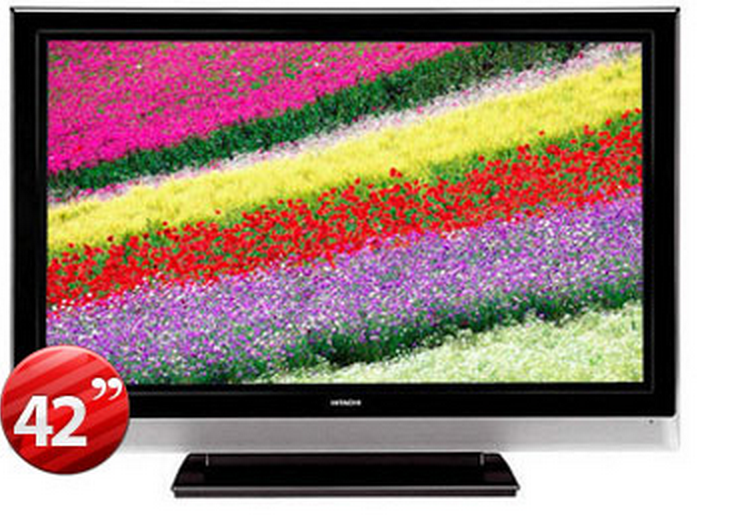
\includegraphics[width=.8\linewidth]{images/fieldSite.png}
	\caption{Image from website}
	\label{fig:example1.1}
\end{minipage}%
\begin{minipage}{.5\textwidth}
	\centering
	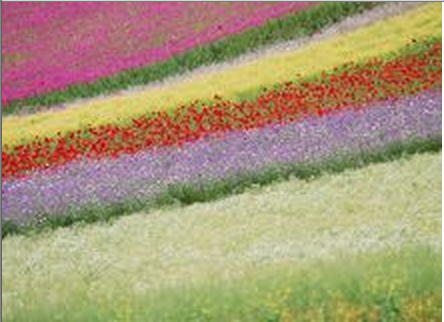
\includegraphics[width=.8\linewidth]{images/field.png}
	\caption{Image from database}
\end{minipage}
\end{figure}

\begin{figure}[ht!]
\centering
\begin{minipage}{.3\textwidth}
	\centering
	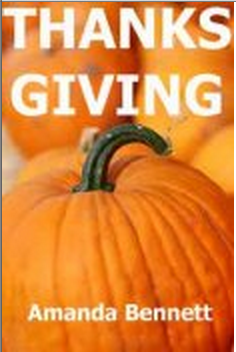
\includegraphics[width=.8\linewidth]{images/pumpkinSite.png}
	\caption{Image from\\ website}
	\label{fig:example2.1}
\end{minipage}%
\begin{minipage}{.3\textwidth}
	\centering
	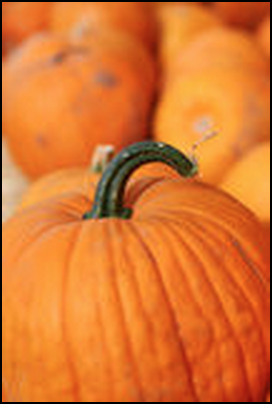
\includegraphics[width=.8\linewidth]{images/pumpkin.png}
	\caption{Image from database}
\end{minipage}
\end{figure}

\section{Running Time}
We have tested our algorithm on a machine with 55GB of RAM, 16 quad-core processors with a frequency of 2.4GHz.\\

\subsection{Comparison between $kdtree\ algorithm$ and $linear\ algorithm$}
The first experiment that we did was comparing the runtimes of the $linear\ algorithm$ with the $kdtree\ algorithm$ by running them on sets of $5, 10, 20, 50, 200, 350$ and $500$ images. The corresponding running times are shown in Figure~\ref{fig:runtimesBasic}.\\
The red line shows the corresponding running times for the $linear\ algorithm$, while the green one shows the times for the $kdtree\ algorithm$. As it can be seen, the $kdtree\ algorithm$ outperformes the linear one, with the same returned image (so it does not give different results). The non-ascending running times of the $kdtree\ algorithm$ can be explained by the fact that the KD-tree data structure is traversed heuristically, so depending on the given input a certain query can execute with varying running times. For a KD-tree of $5000$ images and $5000$ queries, the mean running time of a nearest-neighbor search is $1.36$ seconds.\\
Of course, the $kdtree\ algorithm$ does require an initialization time, which is the price that has to be paid in order to perform fast queries. Figure~\ref{fig:totalRuntimes} shows the sum between the initialization time and query time of a linear image server and an image server which constructs a KD-tree. As it can be seen, the initialization time for the KD-tree grows linearly, but this gets compensated by the small query time. For a $500$-size image set, the initialization and a query on the KD-tree takes $36.771$ seconds, which is less than a query on the same image set using the $linear\ algorithm$, which takes $77.331$ seconds.

\begin{figure}[ht!]
\centering
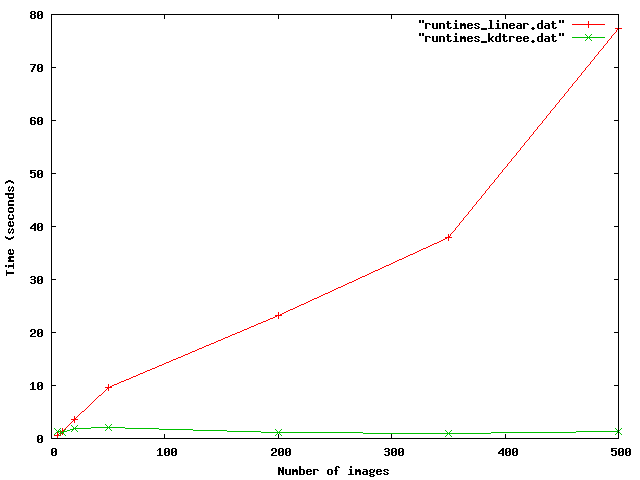
\includegraphics[width=.7\linewidth]{images/runtimesBasic.png}
\caption{Query runtime of the two algorithms}
\label{fig:runtimesBasic}
\end{figure}

\begin{figure}[ht!]
\centering
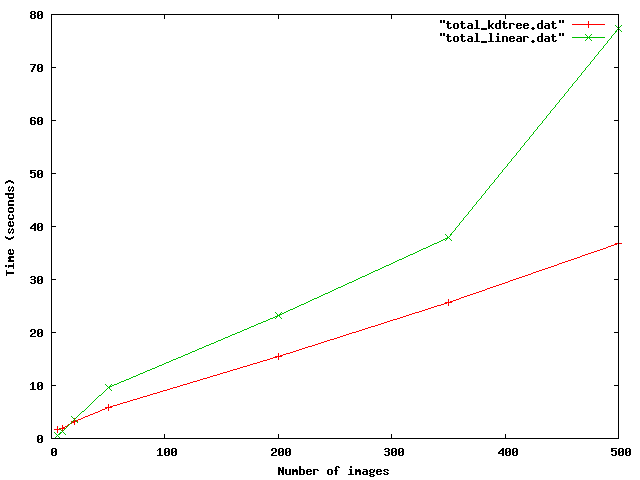
\includegraphics[width=.7\linewidth]{images/totalRuntimes.png}
\caption{Total init and query time for $linear\ algorithm$ and $kdtree\ algorithm$}
\label{fig:totalRuntimes}
\end{figure}

\begin{table}
\centering
\begin{tabular} {c | c | c}
	number of images & $linear\ algorithm$ time & $kdtree\ algorithm$ time \\
	\hline
	5 & 0.60 & 1.391 \\
	10 & 1.23 & 1.21 \\
	20 & 3.54 & 1.90 \\
	50 & 9.58 & 2.08 \\
	200 & 23.28 & 1.05 \\
	350 & 38.00 & 0.96 \\
	500 & 77.33 & 1.39 \\
\end{tabular}
\caption{Query runtime}
\end{table}

\begin{table}
\centering
\begin{tabular} {c | c }
	number of images & $kdtree\ algorithm$ time \\
	\hline
	5 & 1.68 \\
	10 & 1.81 \\
	20 & 3.24 \\
	50 & 5.80 \\
	200 & 15.51 \\
	350 & 25.58 \\
	500 & 36.77 \\
\end{tabular}
\caption{Init and query runtime}
\end{table}



\subsection{Large scale KD-trees}

The second set of tests have been concentrated on analyzing the behavior of large scale KD-trees.
As stated above, our main concern was the initialization time of a KD-tree, which is divided into two steps: the computation of the descriptors for the images, and the construction of the actual KD-tree.\\
In Figure~\ref{fig:totalInit} we can see the total initialization time for a KD-tree, and the time needed only for the construction of the KD-tree data structure (presuming that the descriptors are already computed). \\
\begin{figure}[ht!]
\centering
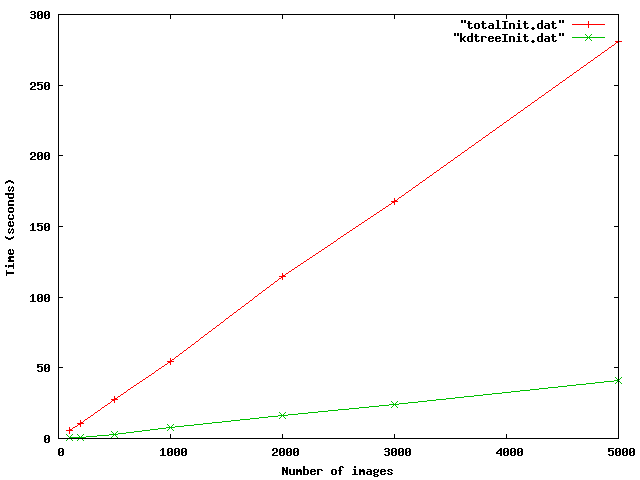
\includegraphics[width=.8\linewidth]{images/totalInit.png}
\caption{Initialization runtimes}
\label{fig:totalInit}
\end{figure}

\begin{table}[H]
\centering
\begin{tabular} {c | c | c}
	number of images & total init (seconds) & kdtree init (seconds) \\
	\hline
	100 & 5.34 & 0.48 \\
	200 & 10.53 & 0.99 \\
	500 & 27.71 & 3.17 \\
	1000 & 54.52 & 7.72 \\
	2000 & 114.27 & 16.26 \\
	3000 & 167.83 & 24.31 \\
	5000 & 280.67 & 41.20 \\
\end{tabular}
\caption{Descriptor computation and KD-tree init time}
\end{table}

Because the total number of images is divided into KD-trees of fixed dimension (in our case $5000$ images), inserting a new image into our database is constant, because it just implies creating a new KD-tree (or expanding a current one, if its dimension doesn't exceed $5000$ images).\\

\subsection{Multiple KD-tree servers}

As shown above, the running time of a nearest-neighbor search is constant, due to its heuristic nature, the overall query time varies depending on the number of processes involved in the search.
This is due to the increasing socket communication between the Map Reducer and the growing number of processes.
We illustrate this overall running time in Figure~\ref{fig:overallTime}, where each process holds a KD-tree of $1000$ images (a higher number of images would not have influenced the process). For each number of processes $20$ queries have been run and the mean execution time of them is listed in table \nameref{table:processTime}, as well as in the figure.\\

\begin{table}[H]
\centering
\begin{tabular} {c | c}
	number of KD-tree servers & query time (seconds) \\
	\hline
	5 & 2.85\\
	10 & 3.24\\
	20 & 3.53\\
	40 & 5.50\\
	60 & 6.38\\
	80 & 8.23\\
	100 & 8.74\\
\end{tabular}
\caption{Execution time for increasing number of KD-tree servers}
\label{table:processTime}
\end{table}

\begin{figure}[H]
\centering
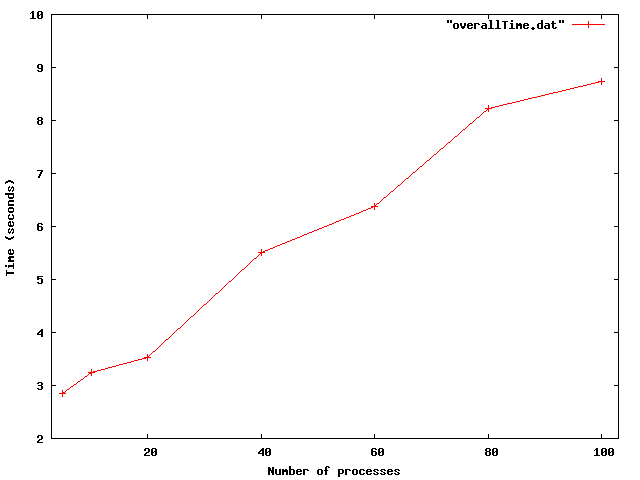
\includegraphics[width=.8\linewidth]{images/overallTime.png}
\caption{Overall query times}
\label{fig:overallTime}
\end{figure}

\subsection{Multi-threaded servers}

As stated in \nameref{chap:implementation}, in order to be able to handle a large number of queries at the same time, the KD-tree servers are multi-threaded, with each separate thread being connected to a different Map Reducer and, thus, being able to support multiple queries simultaneously.\\
Table \ref{table:threadTime} shows the running time for a number of $10$ KD-tree servers, each with $2500$ images and respective number of threads and queries.\\
It can be easily observed that there is a big running time improvement when the number of queries gets bigger and the number of threads increases. In the case of a smaller number of queries, a bigger number of threads does not improve the running time, partially because of the overhead caused by the creation of multiple threads and the overhead of multiple Map Reducers and synchronization between them. \\
Also, because a service with a large number of images will have a considerable amount of Image Servers running (and, implicitly, number of processes), creating more threads will certainly increase the load of the system and not have the desired effect.\\
Inside an Image Server, the KD-tree structure is shared between processes, so, during multiple queries done by multiple threads, the nearest neighbor search performed on the KD-tree may be
a computational bottle neck, all the threads accessing the same data structure.
To avoid this, in case we use multiple KD-trees inside the same Image Server, it could be a good idea to perform the nearest neighbor search in a random order, thus time-multiplexing the access to the data structures.\\

\begin{table}[H]
\centering
\begin{tabular} {c | c | c | c | c}
	\backslashbox{number\\ of threads}{number of\\ queries} & 20 & 50 & 100 & 200 \\
	\hline
	1 & 74.13 & 176.28 & - & - \\
	2 & 38.28 & 94.77 & - & - \\
	3 & 28.15 & 77.51 & - & -\\
	5 & 23.81 & 57.04 & 95.90 & 217.64\\
	10 & - & - & 91.43 & 183.12 \\
	20 & - & - & 90.23 & 180.20 \\
\end{tabular}
\caption{Running time (seconds) for a given number of processes and queries}
\label{table:threadTime}
\end{table}

\subsection{Multiple KD-trees per Image Server}

We analyzed how a certain KD-tree Image Server with a varying number of linear processed KD-trees performs when submitting a query, in order to determine a viable value for the $R$ parameter (the number of KD-trees that form a KD-tree Image Server).\\
In Figure~\ref{fig:multipleKDTrees} and in Table \ref{table:multipleKDTrees} we can observe the running time per query as we increase the number of KD-trees for with $N=2500$ images.\\

\begin{table}[H]
\centering
\begin{tabular}{c | c}
	$R$, number of KD-trees & running time (seconds) \\
	\hline
	2 & 2.45 \\
	3 & 2.75 \\
	5 & 2.84 \\
	10 & 3.01 \\
	20 & 3.44 \\
	40 & 4.41 \\
\end{tabular}
\caption{Running time with various number of KD-trees per KD-tree Image Server}
\label{table:multipleKDTrees}
\end{table}

\begin{figure}[H]
\centering
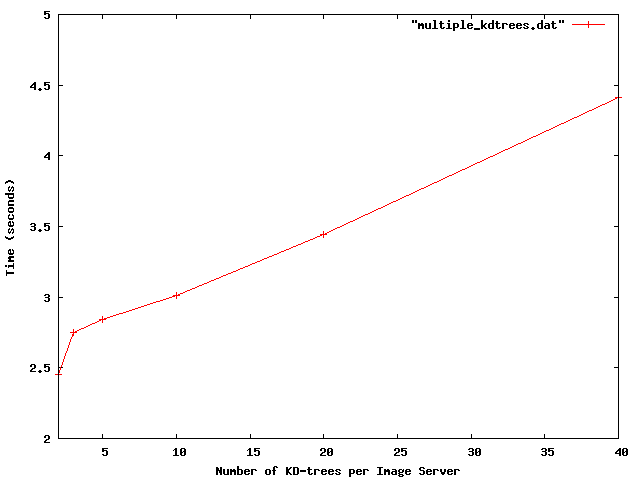
\includegraphics[width=.8\linewidth]{images/multipleKDTrees.png}
\caption{Running time with various number of KD-trees per KD-tree Image Server}
\label{fig:multipleKDTrees}
\end{figure}

By looking at these running times, we can determine that we can easily increase the number of KD-trees per Image Server, as long as we maintain a decent number of images as input for the $linear\ algorithm$, which is used after the actual KD-tree search.\\

\section{Interpretation of results}

By looking both at the running time and correctness of the algorithm, along with the varied parameters which compose it, we have determined the best way to run it when handling a large amount of images:
\begin{itemize}
	\item store images maintaining aspect ratio
	\item store beforehand the computed image descriptors
	\item use the third metric for extracting images from KD-trees: "the images with the largest distance between its descriptors and the average of all found descriptors (from all the images)"
	\item keep a relatively small number of Image Servers
	\item keep a moderate number of threads per Image Server, especially if there isn't a large number of queries
	\item increase the number of KD-trees per Image Server
\end{itemize}
